%
%   section 3
%
%   2018/11/26

\documentclass[11pt,b5paper,papersize,dvipdfmx]{jsbook}

\usepackage{vuccaken}
\usepackage{vuccaken2018}
\usepackage{12nkym}


\begin{document}
% \tableofcontents
% \clearpage

% - - - - - - - - - - - - - - - - - - -
\section{ゼータ関数の解析接続と特殊値}
\label{sec:3}
% - - - - - - - - - - - - - - - - - - -

%
\subsection{複素数版$\zeta(s)$}
%
\begin{thm}{定義&命題(リーマンゼータ関数)}
  複素数$s$について定義されたゼータ関数
  \begin{align}
    \zeta(s) := \sum_{n=1}^\infty \frac{1}{n^s}
    %\equiv \frac{1}{1^s} + \frac{1}{2^s} + \frac{1}{3^s} + \frac{1}{4^s} + \cdots
    \label{eq:zeta-complex}
  \end{align}
  は、$\Re(s) > 1$のとき広義一様に絶対収束し、正則関数となる。また、このような級数による$\zeta(s)$の表示を、ディリクレ級数表示という。
\end{thm}
\begin{prf}
  $\Re(s)>1$のとき$\zeta(s)$が絶対収束することを示す。実数$\sigma,t$を用いて$s\equiv \sigma +it$と書けるとすると、$\zeta(s)$の第$n$項は
  \begin{align*}
    \frac{1}{n^s} &= e^{\log n^{-s}} = e^{-s\log n}\\
    &= e^{-(\sigma +it)\log n}
    = e^{-\sigma \log n} e^{-it\log n}\\
    &= e^{-\sigma \log n} \qty{\cos(t\log n) - i\sin(t\log n)}\\
    &= \frac{1}{n^\sigma } \qty{\cos(t\log n) - i\sin(t\log n)}
  \end{align*}
  であるから、絶対値をとると
  \begin{align*}
    \qty|\frac{1}{n^s}| &= \frac{1}{n^\sigma } \qty|\cos(t\log n) - i\sin(t\log n)|\\
    &= \frac{1}{n^\sigma } \sqrt{\cos[2](t\log n) + \sin[2](t\log n)}\\
    &= \frac{1}{n^\sigma } \qquad (\because \cos^2X + \sin^2X = 1)
  \end{align*}
  となるので、$\dsum_{n=1}^\infty \dfrac{1}{n^\sigma}$が収束すれば$\dsum_{n=1}^\infty \qty|\dfrac{1}{n^s}|$も収束する。
  よって、$s$が実数の場合の議論より、$\zeta(s)$は$\sigma \equiv \Re(s)>1$のとき絶対収束することがわかる。\par
  次に、$\sigma > 1$における収束の広義一様性を示す。$s$が$\Re(s)\equiv \sigma \ge 1+\delta$なる集合内を動くとき、無限和と第$N$部分和の値の差は、次のように評価できる。
  \begin{align*}
    \sum_{n=N}^\infty \frac1{n^\sigma} 
    \le \int_N^\infty \frac1{x^\sigma} \dd{x}
    =\qty[ \frac{x^{1-\sigma}}{1-\sigma} ]_N^\infty
    = \frac1{(\sigma-1) N^{\sigma-1}}
    \le \frac1{\delta N^\delta}
  \end{align*}
  $\dfrac1{\delta N^\delta} < \varepsilon$ なる$N$は$\delta$によってのみ取れ、$s$に依らない。これで広義一様収束であることが示された。
  よって、正則性も従う。
\end{prf}

\subsection{$\zeta(s)$の解析接続}
\label{sec:zeta}
\begin{thm}{定理($\zeta(s)$の解析接続)}
  $\zeta(s)$は、極$s=1$を除く全複素平面$\mathbb{C}$上に解析接続される。
  極$s=1$の位数は$1$であり、留数は$1$である。
\end{thm}
\begin{prf}
  $\Re(s) = \sigma > 1$において、定義式(\ref{eq:zeta-complex})の第1項と第2項を取り分け、第3項から先の無限和と分けて書くと
  \begin{align*}
    \zeta(s) &= 1 + 2^{-s} + \sum_{n=2}^\infty (n+1)^{-s} \\
    &= 1 + 2^{-s} + \sum_{n=2}^\infty n^{-s} \qty(1 + \frac1n )^{-s}
  \end{align*}
  となる。ここで、二項展開
  \begin{align*}
    \qty(1+\frac1n)^{-s} = \sum_{k=0}^\infty \binom{-s}{k} n^{-k}
  \end{align*}
  を用いる。$\binom{-s}{k}$は二項係数
  \begin{align*}
    \binom{-s}{k} = {-s(-s-1)(-s-2)\cdots (-s-k+1) \over k!}
  \end{align*}
  である。すると
  \begin{align*}
    \zeta(s) &= 1 + 2^{-s} + \sum_{n=2}^\infty n^{-s} \sum_{k=0}^\infty \binom{-s}{k} n^{-k}\\
      &= 1 + 2^{-s} + \sum_{n=2}^\infty n^{-s} + \sum_{n=2}^\infty n^{-s} \sum_{k=1}^\infty \binom{-s}{k} n^{-k}\\
      &= \zeta(s) + 2^{-s} + \sum_{n=2}^\infty n^{-s} \sum_{k=1}^\infty \binom{-s}{k} n^{-k}
  \end{align*}
  となる。ここで、$n$と$k$の二重和の順序を交換したい。そのためには順序交換した後の二重級数
  \begin{align*}
    \sum_{k=1}^\infty \binom{-s}{k} \sum_{n=2}^\infty n^{-s-k}
  \end{align*}
  が絶対収束することを示せばよい。まず、$n$にわたる和は
  \begin{align*}
    \sum_{n=2}^\infty \qty|\frac1{n^{s+k}}|
    = \sum_{n=2}^\infty \frac1{n^{\sigma+k}}
    &\le \frac1{2^{\sigma+k}} + \int_2^\infty \frac{\dd{x}}{x^{\sigma+k}}\\
    &= \frac1{2^{\sigma+k}} + \frac1{(\sigma+k-1)2^{\sigma+k-1}}\\
    &< \frac1{2^{k+1}} + \frac1{k2^k}\\
    &\le \frac1{2^{k+1}} + \frac1{2^k}
    = \frac3{2^{k+1}}
  \end{align*}
  のように、$k$に関する公比$\frac12$の等比数列によって評価できるから、
  % のように、$k$に関する公比$\frac12$の等比数列によって評価でき、
  % 二項係数$\binom{-s}{k}$は高々$k$についての多項式であるから、
  $n$にわたる和に二項係数を付けて$k$にわたらせた無限和は絶対収束する。
  よって、上の二重和は順序交換が可能であり
  \begin{align*}
    \zeta(s) &= \zeta(s) + 2^{-s} + \sum_{k=1}^\infty \binom{-s}{k} \sum_{n=2}^\infty n^{-s-k}\\
    &= \zeta(s) + 2^{-s} + \sum_{k=1}^\infty \binom{-s}{k} (\zeta(s+k)-1).
  \end{align*}
  この式から$k=1$を取り出して書くと
  \begin{align*}
    \zeta(s) &= \zeta(s) + 2^{-s} - s(\zeta(s+1)-1)
      + \sum_{k=2}^\infty \binom{-s}{k} (\zeta(s+k)-1)
  \end{align*}
  となる。両辺から$\zeta(s)$を引き、$\zeta(s+1)$について解くと
  \begin{align*}
    \zeta(s+1) = 1 + \frac{2^{-s}}{s} + \frac1s \sum_{k=2}^\infty \binom{-s}{k} (\zeta(s+k)-1)
  .\end{align*}
  $s$と$s-1$に置き換えて
  \begin{align}
    \zeta(s) &= 1 + \frac{2^{1-s}}{s-1} + \frac1{s-1} \sum_{k=2}^\infty \binom{1-s}{k} (\zeta(s-1+k)-1)
    \label{eq:zeta-s>0}\\
    &= 1 + \frac{2^{1-s}}{s-1} + \frac{s}{2}(\zeta(s+1)-1)
      - \frac{s(s+1)}{6}(\zeta(s+2)-1) \notag
  \end{align}
  となる。この置き換えによって、これまで$\Re(s)>1$としていた仮定が$\Re(s)>2$となったが、ここで(\ref{eq:zeta-s>0})の両辺の各々がより広い範囲の$s$で定義されるかどうかみてみる。 \par 
  右辺に現れる全項のゼータ関数は$\Re(s)>0$において定義されるから、$k$にわたる無限和は$\Re(s)>0$において絶対収束し、極限として得る関数は正則となる。よって、左辺の$\zeta(s)$の定義域は、$s=1$の極を除いて$\Re(s)>0$にまで拡張されたことになる。このように一度定義域が広がれば、あとは(\ref{eq:zeta-s>0})を繰り返し用いて複素平面全体への解析接続ができる。\par
  また、(\ref{eq:zeta-s>0})の表示から、極は$s=1$のみであり、位数は$1$で留数は
  \begin{align*}
    \lim_{s\to 1} (s-1) \frac{2^{1-s}}{s-1} = 1
  \end{align*}
  と求められる。
\end{prf}

\clearpage

%
\subsection{特殊値$\zeta(0)$}
上で与えた$\zeta(s)$の解析接続の証明は初等的なものであるが、特殊値を容易に計算できるという利点がある。
\begin{thm}{定理}
  \begin{align}
    \zeta(0) = -\frac12.
  \end{align}
\end{thm}
\begin{prf}
  (\ref{eq:zeta-s>0})の表示において$s\to 0$とすると
  \begin{align*}
    \zeta(0) &= 1 + \frac{2}{-1} + \frac12 \lim_{s\to 0} s\,\zeta(s+1)\\
    &= 1 - 2 + \frac12 = -\frac12
  \end{align*}
\end{prf}

これで目標のひとつ、特殊値$\zeta(0)$の値を知ることができた。
あとは微分係数$\zeta'(0)$を求めるために、表示(\ref{eq:zeta-s>0})を微分して$s\to 0$とすれば...と思ったが、この表示を実際に微分して$\zeta'(0)$を求めるのは容易ではなさそうだ。少なくとも私には無理だった(できそうな人はトライしてみてください)。ということで、このダイレクトな方法は諦め、イータ関数$\eta(s)$を使った方法で求めることにする。道のりは長いが、こちらの方が確実である
\footnote{これから行う方法はあまり一般的なものではないらしい。アダマール積だとかフォン・マンゴールド関数を使った方法がよく見られる。しかしまあ既に調べてしまったものは仕方ないので、別の方法は各自ググってもらうとしよう。}。



% - - - - - - - - - - - - - - - - - - - -
\subsection{特殊値$\zeta'(0)$}
\label{sec:zeta'(0)}
% - - - - - - - - - - - - - - - - - - - -

前のセクションで$\zeta(s)$を解析接続するとすぐに$\zeta(0)$の値も求まったが、$\zeta'(0)$の値はそう簡単にはいかない。これで最後なので頑張ろう。

\begin{thm}{定義&命題(ディリクレのイータ関数)}
  複素数$s$について、無限級数によって定義された関数
  \begin{align}
    \eta(s) := \sum_{n=1}^\infty \frac{(-1)^{n-1}}{n^s}
    \equiv \frac{1}{1^s} - \frac{1}{2^s} + \frac{1}{3^s} - \frac{1}{4^s} + \cdots
  \end{align}
  は、$\Re(s)>1$のとき広義一様に絶対収束し、正則関数となる。また、$\eta(s)$はディリクレのイータ関数と呼ばれる。
\end{thm}
\begin{prf}
  $\eta(s)$は$\zeta(s)$の交代級数であるから、絶対収束性についての議論は$\zeta(s)$と同じ。
\end{prf}

\begin{thm}{定理(イータ関数とゼータ関数の関係式)}
  $\Re(s)>1$の領域において
  \begin{align}
    \eta(s) = (1 - 2^{1-s})\zeta(s) \label{eq:eta-zeta}
  \end{align}
  という関係式が成り立つ。
\end{thm}
\begin{prf*}
  $\Re(s)>1$とすると、絶対収束する領域では項の順序を入れ替えても良いので
  \begin{align*}
    \eta(s) &= 1 - \frac1{2^s} + \frac1{3^s} - \frac1{4^s} + \cdots\\
    &= \qty(1 + \frac1{2^s} + \frac1{3^s} + \frac1{4^s} + \cdots)
      - 2\qty(\frac1{2^s} + \frac1{4^s} + \cdots)\\
    &= \sum_{n=1}^\infty \frac{1}{n^s} - 2\sum_{n=1}^\infty \frac{1}{(2n)^s}\\
    &= \sum_{n=1}^\infty \frac{1}{n^s} - 2\cdot 2^{-s} \sum_{n=1}^\infty \frac{1}{n^s}\\
    &= (1 - 2^{1-s}) \sum_{n=1}^\infty \frac{1}{n^s}
    = (1 - 2^{1-s}) \zeta(s).
  \end{align*}
\end{prf*}

(\ref{eq:eta-zeta})式から$\eta(s)$は$s=1$を除いた複素数全体へ解析接続されることがすぐにわかる。
$s=1$では$\eta(1)=0\cdot\infty$となり不定形であるが、これは$\log2$という値に収束することが知られている
\footnote{
  直感的には、
  $|x|<1$において収束する$\log(1+x)$のテイラー展開
  \begin{align*}
    \log(1+x) = x - \frac{x^2}{2} + \frac{x^3}{3} - \frac{x^4}{4} + \cdots
  \end{align*}
  において$x=1$とすれば$\eta(1)=\log2$を得ることができる。
}。
$\eta(s)$は$s=1$でも有限値をとるので、複素数平面全体で正則な関数に解析接続できるのかな? まあ今回は$s=1$はどうでもいいので、とりあえず先に進もう。


\begin{thm}{定理(イータ関数の別表示)}
  \begin{align}
    \eta(s) = \frac12 + \frac12 \sum_{n=1}^\infty (-1)^{n-1} \{n^{-s} - (n+1)^{-s}\} \label{eq:eta-other}
  \end{align}
\end{thm}
\begin{prf}
  \noindent
  \begin{align*}
    \eta(s) &= 1 - 2^{-s} + 3^{-s} - 4^{-s} + \cdots \\
    &= \frac12 \,( 1 + 1 - 2^{-s} - 2^{-s} + 3^{-s} + 3^{-s} - 4^{-s} - \cdots )\\
    &=  \frac12 + \frac12 \,( 1 - 2^{-s} - 2^{-s} + 3^{-s} + 3^{-s} - 4^{-s} - \cdots )\\
    &= \frac12 + \frac12 \,\qty{(1 - 2^{-s}) - (2^{-s} - 3^{-s}) + (3^{-s} - 4^{-s}) - \cdots }\\
    &= \frac12 + \sum_{n=1}^\infty (-1)^{n-1} \qty{ n^{-s} - (n+1)^{-s} }
  \end{align*}
\end{prf}

\begin{thm}{定理(余接関数の極)}
  $\cot z \equiv \dfrac{\cos z}{\sin z}$は、$z=\pi n \quad (n \in \mathbb{Z})$に1位の極を持ち、それらの留数はすべて1である。
\end{thm}
\begin{prf}
  $z\equiv x+iy\quad (x,y\in\mathbb{R})$とすると
  \begin{align*}
    \sin z &= \sin(x+iy)\\
    &= \sin x \cos(iy) + \cos x \sin(iy)\\
    &= \sin x \cosh y + i\cos x \sinh y
  \end{align*}
  であるから
  \begin{align*}
    \sin z = 0 
    &\iff \text{$\sin x \cosh y = 0$ かつ $\cos x \sinh y = 0$}\\
    &\iff \text{$\sin x = 0$ かつ「$\cos x = 0$ または $\sinh y = 0$」}\\
    &\iff \text{$x=\pi n$ かつ「$x=\frac{\pi n}{2}\,\,(n\ne 0) $ または $y=0$」}\\
    &\iff \text{$x=\pi n$ かつ $y=0$}\\
    &\iff z = \pi n
  \end{align*}
  である。$z = \pi n$で$\cos z \ne 0$なので、$\cot z$の極は$\sin z$の零点と一致し、$z = \pi n$のみであることがわかる。
  また
  \begin{align*}
    \lim_{z\to\pi n} (z-\pi n)\cot z
    &= \lim_{z\to\pi n} (z-\pi n) \frac{\cos z}{\sin z}\\
    &= \lim_{A \to 0} A\cdot\frac{\cos(A+\pi n)}{\sin(A+\pi n)}\\
    &= \lim_{A \to 0} A\cdot\frac{\cos{A}\cos{\pi n} - \sin{A}\sin{\pi n} }{\sin{A}\cos{\pi n} + \cos{A}\sin{\pi n} }\\
    &= \lim_{A \to 0} \frac{A}{\sin A} \cdot \cos A = 1
  \end{align*}
  であるから、すべての極$z=\pi n$の位数は1であり、留数は1である。
\end{prf}


\begin{thm}{定理(余接関数の部分分数展開)}
  \begin{align}
    \cot z = \frac1z + \sum_{n=1}^\infty \frac{2z}{z^2 - \pi^2 n^2}
    \label{eq:cot}
  \end{align}
\end{thm}
\begin{prf}
  (\ref{eq:cot})を証明するためには、図\ref{fig:cot}のように経路$C$に沿った積分
  \begin{align*}
    \oint_C \frac{\cot \zeta}{\zeta(\zeta-z)}\dd{\zeta}
    \quad (z \ne \pi n)
  \end{align*}
  を2つの方法で計算すればよい。すなわち、(i)留数定理を使う方法と、
  (ii)積分を直接実行する方法で求めた積分値が等しいとおく。\par
  %
  \begin{figure}[H]
    \centering
    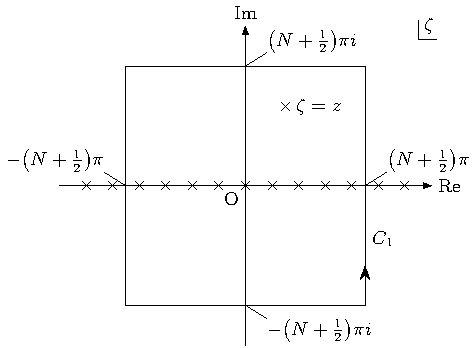
\includegraphics{nkym/fig/cot.pdf}
    \caption{経路$C$と$\dfrac{\cot\zeta}{\zeta(\zeta-z)}$の極}
    \label{fig:cot}
  \end{figure}
  %
  (i)まず$\dfrac{(\cot \zeta)}{\zeta(\zeta-z)}$は$\zeta = z$と$\zeta = \pi n$のところに極を持つ。
  $\zeta = z$と$\zeta = \pi n \,\,(n \ne 0)$のところは1位の極であり、
  留数はそれぞれ$\dfrac{\cot z}z$と$\dfrac1{\pi n(\pi n - z)}$である。
  $\zeta = 0$のところは2位の極であり、留数は
  \begin{align*}
    &\lim_{\zeta\to0}\dv{\zeta}\qty(\zeta^2\cdot \frac{\cot \zeta}{\zeta(\zeta-z)})
    = \lim_{\zeta\to0}\dv{\zeta}\qty(\frac{\zeta \cot \zeta}{(\zeta-z)})\\
    &= \lim_{\zeta\to0}\qty( \frac{\cot \zeta}{\zeta-z} - \frac{\zeta}{(\zeta-z)\sin^2\zeta} - \frac{\zeta\cot\zeta}{(\zeta-z)^2} )\\
    &= \lim_{\zeta\to0}\qty( \frac{\cos\zeta}{\zeta(\zeta-z)}\frac{\zeta}{\sin\zeta} - \frac{1}{\zeta(\zeta-z)}\frac{\zeta^2}{\sin^2\zeta} - \frac{\cos\zeta}{(\zeta-z)^2}\frac{\zeta}{\sin\zeta} )\\
    &= \lim_{\zeta\to0}\qty( \frac{1}{\zeta(\zeta-z)} - \frac{1}{\zeta(\zeta-z)} - \frac{1}{(\zeta-z)^2} )\\
    &= \lim_{\zeta\to0}\qty( -\frac{1}{(\zeta-z)^2} )
    = - \frac1{z^2}
  \end{align*}
  と求まる。よってこれらの留数を合計すると積分値が求まり
  \begin{align}
    \oint_C \frac{\cot \zeta}{\zeta(\zeta-z)}\dd{\zeta}
    = 2\pi i \qty\Bigg(\frac{\cot z}{z} + \sum_{\substack{n=-N \\ n\ne0}}^N \frac1{\pi n(\pi n-z)} -\frac1{z^2})
    \label{eq:cot-sum}
  \end{align}
  となる。\par
  %
  (ii)次に(\ref{eq:cot-sum})式左辺の積分を経路$C$の各辺ごとに実行してみる。例えば図\ref{fig:cot}の右辺部分の経路$C_1$に沿った積分は$\zeta = (N+\frac12)\pi + iy$とおいて
  \begin{align*}
    \int_{C_1} \frac{\cot \zeta}{\zeta(\zeta-z)}\dd{\zeta}
    = \int_{-\qty(N+\frac12)\pi}^{\qty(N+\frac12)\pi}
      { \cot\qty{\qty(N+\frac12)\pi+iy} \over 
      \qty{\qty(N+\frac12)\pi+iy} \qty{\qty(N+\frac12)\pi+iy-z} } \,i\dd{y}
  \end{align*}
  であるが
  \begin{align*}
    \textstyle \qty| \cot\qty{\qty(N+\frac12)\pi + iy} |
    &= \qty|{ \sin(N+\frac12)\pi \cdot \sin iy + \cos(N+\frac12)\pi \cdot \cos iy \over \sin(N+\frac12)\pi \cdot \cos iy + \cos(N+\frac12)\pi \cdot \sin iy }|\\
    &= \qty|{\sin iy \over \cos iy }|
    = \qty|{ e^{-y} - e^y \over e^{-y} + e^y }| \le 1
  \end{align*}
  であり、また$-(N+\frac12)\pi \le y \le (N+\frac12)\pi $において
  \begin{align*}
    \qty|\qty(N+\tfrac12)\pi+iy|
    = \sqrt{ \qty{\qty(N+\tfrac12)\pi}^2 + y^2 }
    \ge \qty(N+\tfrac12)\pi,\\
    \qty|\qty(N+\tfrac12)\pi+iy-z|
    \ge \qty|\qty(N+\tfrac12)\pi+iy|-|z|
    \ge \qty(N+\tfrac12)\pi -|z|
  \end{align*}
  であるから
  \begin{align*}
    \qty| \int_{C_1} \frac{\cot \zeta}{\zeta(\zeta-z)}\dd{\zeta} |
    &\le \int_{-\qty(N+\frac12)\pi}^{\qty(N+\frac12)\pi}
      \qty| { \cot\qty{\qty(N+\frac12)\pi+iy} \over 
      \qty{\qty(N+\frac12)\pi+iy} \qty{\qty(N+\frac12)\pi+iy-z} } | \dd{y}\\
    &\le \int_{-\qty(N+\frac12)\pi}^{\qty(N+\frac12)\pi}
      \frac1{ \qty(N+\frac12)\pi \qty{\qty(N+\frac12)\pi-|z|} } \dd{y}\\
    &= \frac2{ \qty(N+\frac12)\pi - |z| }.
  \end{align*}
  したがって、$N\to\infty$のとき積分値は$0$に近づく
    % \footnote{
    %   直感的には次のように理解すれば簡単である。
    %   経路$C$上において、$\cot(x+iy)$は$x=0$のところに位数1の極を持つだけで、他の点では有限である。よって$N\to\infty$で
    %   \begin{align*}
    %     \qty| \oint_{C} \frac{\cot \zeta}{\zeta(\zeta-z)}\dd{\zeta} |
    %     = \frac{\infty}{\infty\times\infty}
    %     = \frac1\infty = 0
    %   \end{align*}
    %   となる。
    % }
  。他の部分の経路からの寄与も同じように小さくなるので、結局(\ref{eq:cot-sum})式左辺は$N\to\infty$で$0$である。つまり
  \begin{align*}
    \frac{\cot z}{z} + \sum_{\substack{n=-\infty \\ n\ne0}}^\infty \frac1{\pi n(\pi n-z)} -\frac1{z^2} = 0
  \end{align*}
  が成立する。この式を整理すると
  \begin{align*}
    \cot z &= \frac1z - \sum_{\substack{n=-\infty \\ n\ne0}}^\infty \frac{z}{\pi n(\pi n-z)}\\
    &= \frac1z - \sum_{n=1}^\infty 
      \qty{ \frac{z}{\pi n(\pi n-z)} + \frac{z}{-\pi n(-\pi n-z)} }\\
    &= \frac1z + \sum_{n=1}^\infty \frac{2z}{z^2 - \pi^2 n^2}
  \end{align*}
  となる。
%
\end{prf}


\begin{thm}{定理(サイン関数の無限積展開)}
  \begin{align}
    \sin z = z \prod_{n=1}^\infty \pqty{1 - \frac{z^2}{\pi^2 n^2}}
    \label{eq:sin-prod}
  \end{align}
\end{thm}
\begin{prf}
  まず任意の複素数$z$を固定するとき、級数$ \dsum_{n=1}^\infty \qty\Big(-{ \dfrac{z^2}{n^2}}) $は広義一様に絶対収束するので、無限積$P(z) := \dprod_{n=1}^\infty \pqty\Big{1 - \dfrac{z^2}{\pi^2 n^2}}$も広義一様に絶対収束し、正則関数となる。
  そこで、関数$f(z)$を
  \begin{align*}
    f(z) := \frac{ z P(z) }{\sin z}
  \end{align*}
  と定義し、これが恒等的に$f(z) \equiv 1$であることを示せばよい。
  両辺対数をとると
  \begin{align*}
    \log f(z) = \log z + \sum_{n=1}^\infty \qty[ \log(1+\frac{z}{\pi n}) + \log(1-\frac{z}{\pi n}) ] - \log(\sin z)
  \end{align*}
  であり、微分すると
  \begin{align*}
    \dv{z}\log f(z) &= \frac1z + \sum_{n=1}^\infty \qty[ \frac1{1+\frac{z}{\pi n}} - \frac1{1-\frac{z}{\pi n}} ] - \frac{\cos z}{\sin z}\\
    &= \frac1z + \sum_{n=1}^\infty \frac{2z}{z^2-n^2} - \cot z.
  \end{align*}
  ここで(\ref{eq:cot})より
  \begin{align*}
    \dv{z}\log f(z) = 0
  \end{align*}
  となる。よって
  \begin{align*}
    \log f(z) &= \text{\const}\\
    f(z) &= \text{\const}
  \end{align*}
  となるから、$\displaystyle \lim_{z \to 0} \frac{z}{\sin z} = 1$に注意して
  \begin{align*}
    f(z) \equiv f(0) = \lim_{z \to 0} \frac{zP(z)}{\sin z}
    = P(0) = 1.
  \end{align*}
\end{prf}

%
なお、$\sin z$の無限積展開は、多項式にしか使えない因数定理を誤用することでも奇跡的に求められる。すなわち、$\sin z$が零点$z=\pi n \,\, (n\in\mathbb{Z})$を持つことから
\begin{align*}
  \sin z &= az(z+\pi)(z-\pi)(z+2\pi)(z-2\pi)(z+3\pi)(z-3\pi)\cdots\\
  &= az \prod_{n=1}^\infty (z+n\pi)(z-n\pi)
\end{align*}
というように因数分解できるとする。係数$a$を決定するために両辺$z$で割り$z\to0$とすると
\begin{align*}
  1 = \lim_{z\to0} \frac{\sin z}{z}
  = a \prod_{n=1}^\infty n\pi(-n\pi)
\end{align*}
であるから
\begin{align*}
  a = \prod_{n=1}^\infty \frac1{n\pi(-n\pi)}.
\end{align*}
よって
\begin{align*}
  \sin z &= z \prod_{n=1}^\infty \frac{(z+n\pi)(z-n\pi)}{n\pi(-n\pi)}\\
  &= z \prod_{n=1}^\infty \qty(1+\frac{z}{n\pi}) \qty(1-\frac{z}{n\pi})\\
  &= z \prod_{n=1}^\infty \qty(1-\frac{z^2}{n^2 \pi^2})
\end{align*}
となり、上で示したことと同じ結果が得られた。
これはかの天才オイラーによって発見された方法であり、オイラーはさらに$\sin z$のマクローリン展開
\begin{align*}
  \sin z = z - \frac{z^3}{3!} + \frac{z^5}{5!} - \frac{z^7}{7!} + \cdots
\end{align*}
と上で示した$\sin z$の無限積表示の$z^3$の係数を比較することで、
\begin{align}
  \zeta(2) = \sum_{n=1}^\infty \frac1{n^2} = \frac{\pi^2}{6}
\end{align}
であることを示し、バーゼル問題を解決した。\par
天才オイラーの登場によって話が逸れてしまったが、ここで話を戻し、$\sin z$の無限積展開の特殊値としてウォリス積というものを求めよう。
%

\begin{thm}{定理(ウォリス積)}
  \begin{align}
    \frac{\pi}{2} &= \prod_{n=1}^\infty \frac{(2n)^2}{(2n-1)(2n+1)}
    \label{eq:wallis}\\
    &\equiv \frac{2\cdot 2}{1\cdot 3}\cdot \frac{4\cdot 4}{3\cdot 5}\cdot \frac{6\cdot 6}{5\cdot 7}\cdot \cdots \notag
  \end{align}
\end{thm}
\begin{prf}
  (\ref{eq:sin-prod})において$\displaystyle z=\frac\pi2$を代入すると
  \begin{align*}
    \sin \frac\pi2 &= \frac\pi2 \prod_{n=1}^\infty \pqty{1 - \frac{1}{4n^2}}\\
    1 &= \frac\pi2 \prod_{n=1}^\infty \pqty{ \frac{(2n)^2 - 1}{(2n)^2} }\\
    &= \frac\pi2 \prod_{n=1}^\infty \frac{(2n-1)(2n+1)}{(2n)^2}\\
    \frac\pi2 &= \prod_{n=1}^\infty \frac{(2n)^2}{(2n-1)(2n+1)}.
  \end{align*}
\end{prf}

これでようやく$\zeta'(0)$を求める準備が整った。これで本当に最後なので頑張っていこう。

\begin{thm}{定理}
  \begin{align}
    \zeta'(0) = -\frac12 \log 2\pi
  \end{align}
\end{thm}
\begin{prf}
  (\ref{eq:eta-zeta}),\,(\ref{eq:eta-other})より
  \begin{align*}
    (1 - 2^{1-s}) \zeta(s) = \frac12 + \sum_{n=1}^\infty (-1)^{n-1} \qty{ n^{-s} - (n+1)^{-s} }
  \end{align*}
  ここで、両辺$s$で微分し、$s=0$を代入する。\par
  右辺については
  \begin{align*}
    \dv{x} a^{-x} = \dv{x} e^{-x\log a} = -a^{-x}\log a
  \end{align*}
  であることに注意して
      \par
  \begin{align*}
    \eval{\dv{s}(右辺)}_{s=0}
    &= \eval{ \frac12 + \sum_{n=1}^\infty (-1)^n \qty{ \frac{\log n}{n^s} - \frac{\log(n+1)}{(n+1)^s} }}_{s=0}\\
    &= \frac12 + \sum_{n=1}^\infty (-1)^n \qty{ \log n- \log(n+1) }\\
    &= \frac12 \,\qty{ -(\log1 -\log2) +(\log2 -\log3) -(\log3-\log4) +\cdots }\\
    &= \frac12 \log\qty{ \frac{2\cdot 2\cdot 4\cdot 4\cdot 6\cdot 6\cdots}{1\cdot 3\cdot 3\cdot 5\cdot 5\cdot 7\cdots} }\\
    &= \frac12 \log \prod_{n=1}^\infty \frac{(2n)^2}{(2n-1)(2n+1)}\\
    &= \frac12 \log\frac\pi{2}
  \end{align*}
  となる。ただし最後の変形でウォリス積(\ref{eq:wallis})式を用いた。\par
  一方、左辺については、既に求めた特殊値$\zeta(0)=-\frac12$を用いて
  \begin{align*}
    \eval{\dv{s}(左辺)}_{s=0}
    &= \eval{ 2^{1-s}\log2 \cdot \zeta(s) + (1 - 2^{1-s}) \zeta'(s) }_{s=0}\\
    &= 2\log2 \cdot \zeta(0) - \zeta'(0)\\
    &= -\log2 - \zeta'(0)
  \end{align*}
 となる。よって両辺等しいのだから
 \begin{align*}
    \frac12 \log\frac\pi{2} &= -\log2 - \zeta'(0)\\
    \zeta'(0) &= \frac12 \log\frac\pi{2} + \log2\\
    &= \frac12 \log 2\pi.
 \end{align*} 
\end{prf}

以上より、ゼータ関数の特殊値$\zeta(0)$および$\zeta'(0)$を求めることができた。
ここまで道のりが長いと何のためにゼータ関数の特殊値を計算したのか忘れてしまいそうだが、これでようやく
\begin{align*}
  2\times 3\times 5\times 7\times 11\times\cdots = 4\pi^2
\end{align*}
という数式を理解できたと言っても良いだろう。\par

目的は全て達成されもうお腹もいっぱいなのでここで終わっても良いのだが、せっかくゼータ関数$\zeta(s)$とお友達になって(定義して)さらには親友にもなった(解析接続もした)ので、かの有名な未解決問題「リーマン予想」に触れない手はない。\par
以降のセクションでは、リーマン予想を証明することはないが、それがどんなものであるか、何が面白いのかについて簡単に説明し、リーマン予想が正しいことを支持する数値計算の結果を見せる。\par

それではここで 
\begin{quote}
  リーマンの奇妙な冒険 第一部 完
\end{quote}
とする。


%%%%%%
\end{document}
